%{{{ Formatierung

\documentclass[a4paper,12pt]{article}

\usepackage{physics_notetaking}

%%% dark red
%\definecolor{bg}{RGB}{60,47,47}
%\definecolor{fg}{RGB}{255,244,230}
%%% space grey
%\definecolor{bg}{RGB}{46,52,64}
%\definecolor{fg}{RGB}{216,222,233}
%%% purple
%\definecolor{bg}{RGB}{69,0,128}
%\definecolor{fg}{RGB}{237,237,222}
%\pagecolor{bg}
%\color{fg}

\newcommand{\td}{\,\text{d}}
\newcommand{\RN}[1]{\uppercase\expandafter{\romannumeral#1}}
\newcommand{\zz}{\mathrm{Z\kern-.3em\raise-0.5ex\hbox{Z} }}
\newcommand{\id}{1\kern-.258em1}

\newcommand\inlineeqno{\stepcounter{equation}\ {(\theequation)}}
\newcommand\inlineeqnoa{(\theequation.\text{a})}
\newcommand\inlineeqnob{(\theequation.\text{b})}
\newcommand\inlineeqnoc{(\theequation.\text{c})}

\newcommand\inlineeqnowo{\stepcounter{equation}\ {(\theequation)}}
\newcommand\inlineeqnowoa{\theequation.\text{a}}
\newcommand\inlineeqnowob{\theequation.\text{b}}
\newcommand\inlineeqnowoc{\theequation.\text{c}}

\renewcommand{\refname}{Source}
\renewcommand{\sfdefault}{phv}
%\renewcommand*\contentsname{Contents}

\pagestyle{fancy}

\sloppy

\numberwithin{equation}{section}

%}}}

\begin{document}

%{{{ Titelseite

\title{3/4 (1. Halbtag) $|$ Transistor und Transistorverstärker}
\author{Angelo Brade, Jonas Wortmann}
\maketitle
\pagenumbering{gobble}

%}}}

\newpage

%{{{ Inhaltsverzeichnis

\fancyhead[L]{\thepage}
\fancyfoot[C]{}
\pagenumbering{arabic}

\tableofcontents

%}}}

\newpage

%{{{

\fancyhead[R]{\leftmark}

\section{Einleitung}
jjj

\clearpage
\section{Theorie}

\clearpage
\section{Voraufgaben}
\subsection{A}
\begin{figure}[h]
        \centering
        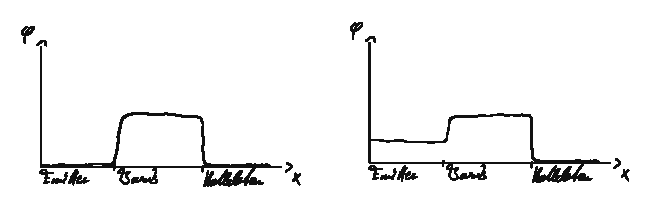
\includegraphics[width=0.9\textwidth]{A_crop.pdf}
        \caption[Potentialverlauf ohne und mit äußerer Spannung]{Potentialverlauf ohne (links) und mit (rechts) äußerer Spannung}
\end{figure}

\subsection{B}
Im Emitter ist eine hohe Elektronendichte; in der Basis ist nur eine geringe Löcherdichte; im Kollektor ist eine weniger starke Elektronendichte als im Emitter.

\subsection{C}
Es gilt 
\begin{align} 
        I_E&=I_B+I_C&\beta &=\diff[]{I_C}{I_B}&\alpha &=\diff[]{I_C}{I_E}&\gamma &=\diff[]{I_E}{I_B}
.\end{align} 
Leitet man nach $I_B$ ab folgt 
\begin{align} 
        &&\diff[]{I_E}{I_B}&=\diff[]{I_B}{I_B}+\diff[]{I_C}{I_B}&&\\
        \Leftrightarrow &&\gamma &=1+\beta .&&
\end{align} 
Leitet man nach $I_E$ ab folgt
\begin{align} 
        &&\diff[]{I_E}{I_E}&=\diff[]{I_B}{I_E}+\diff[]{I_C}{I_E}&&\\
        \Leftrightarrow &&1&=\dfrac{1}{\gamma }+\alpha &&\nonumber \\
        \Leftrightarrow &&\dfrac{1}{1-\alpha }&=\gamma &&\nonumber \\
        \Leftrightarrow &&\dfrac{1}{1-\alpha }-1&=\beta &&\nonumber \\
        \Leftrightarrow &&\dfrac{\alpha }{1-\alpha }&=\beta .&&
\end{align} 


\clearpage
\section{Auswertung}

\clearpage
\listoffigures
\listoftables
\bibliographystyle{plain}
\bibliography{refs}

%}}}

\end{document}
